\SourceLeaf{168}gelingt, alle Hindernisse zu überwinden. Ich würde dann mit der
innigsten Freude alles tun, um Dein Verdienst zur Geltung zu bringen und
ins rechte Licht zu stellen, soweit es in meinen Kräften steht. Ich komme nun
gleich zur Sache.

Gegen alle \textls{übrigen} Schlüsse habe ich nichts Wesentliches
einzuwenden. Was mich \textls{nicht} 
überzeugt hat, ist allein die Argumentation in Artikel XIII. Du denkst
Dir dort eine ins Unbestimmte fortgeführte Linie $\Pi\dots kdcfg\dots$,
die aus lauter geraden und gleich langen Stücken besteht, $kd$, $dc$, $cf$,
$fg$ usw., und bei der die Winkel $kdc$, $dcf$, $cfg$ usw. einander gleich
sind. Du willst beweisen, dass $\Pi$ früher oder später notwendig
über $k\varphi$ hinausgehen werde. Dazu lässt Du die
gerade Linie $kd\infty = Q$ nach der Seite, auf der $\Pi$ liegt,
um $k$ rotieren, sodass sie nach und nach von einer Seite des
Polygons $\Pi$ zur nächsten gelangt. Du zeigst ausgezeichnet, dass $Q$,
wenn es nacheinander durch $d, c, f, g$ usw. geht, jedes Mal näher
an $k\varphi$ kommt. Dagegen lässt sich
\textls{Nichts} 
einwenden. Nun fährst Du aber fort
\begin{center}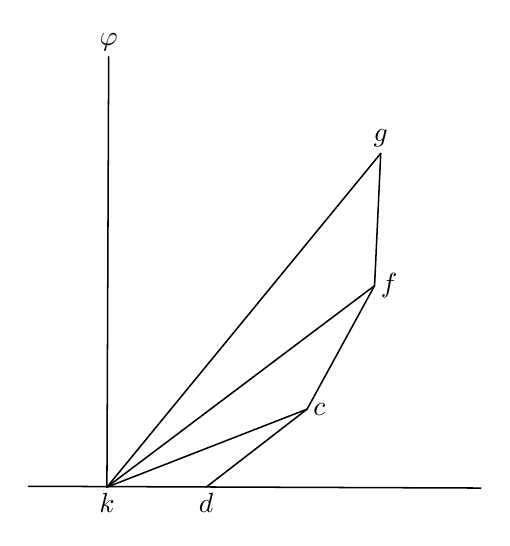
\begin{tikzpicture}[x=1.12cm,y=1.12cm,line width=.55pt,line cap=round,line join=round]
\coordinate (k) at (0,0);
\coordinate (d) at (1.125,0);
\coordinate (c) at (2.27,.885);
\coordinate (f) at (3.035,2.285);
\coordinate (g) at (3.105,3.785);
\coordinate (phi) at (.02,4.88);
\draw (-.89,.01)--(4.24,-.01);
\draw (k)--(phi);
\draw (k)--(c);
\draw (k)--(f);
\draw (k)--(g);
\draw (d)--(c)--(f)--(g);
\node[above,inner sep=2pt] at (phi) {$\varphi$};
\node[above,inner sep=2pt] at (g) {$g$};
\node[right,inner sep=2pt] at (f) {$f$};
\node[right,inner sep=2pt] at (c) {$c$};
\node[below,inner sep=2pt] at (d) {$d$};
\node[below,inner sep=2pt] at (k) {$k$};
\end{tikzpicture}
\end{center}
\begin{quote}
»Quapropter $Q$ moveri potest modo praescripto usque dum in
$k\varphi$, $\varphi\infty$ pervenerit« etc.
\end{quote}
und diese Folgerung leuchtet mir nicht ein. Aus Deiner
Argumentation folgt meiner Ansicht nach noch gar nicht, dass der
Winkel, um den $Q$ beim Durchlaufen einer Seite von $\Pi$ (nach oben
herum) $k\varphi$ näher kommt, nicht etwa immer kleiner
wird, sodass die Summe aller aufeinanderfolgenden Annäherungen, so oft
sie auch wiederholt werden, dennoch nie groß [genug]
werden könnte, um $Q$ in $k\varphi$ zu bringen. Könntest Du \textls{beweisen},
dass $dkc = ckf = fkg$ usw., so wäre die Sache sogleich geklärt.
Dieser Satz ist zwar wahr, aber schwerlich streng zu beweisen, ohne
die Theorie der Parallelen bereits vorauszusetzen. Man könnte
also immer noch befürchten, dass die Winkel $dkc$, $ckf$, $fkg$ usw.
nacheinander abnehmen. Geschähe dies (bloß \textls{zum Beispiel}) in einer
geometrischen Progression, sodass $ckf = \psi \times dkc$,
$fkg = \psi \times dkc$ usw. (sodass $\psi$ kleiner als 1), so würde
